\documentclass[fleqn, 10pt]{article}

% Paquetes necesarios
\usepackage[utf8]{inputenc}
\usepackage{amsthm, amsmath}
\usepackage{nccmath} %Para centrar ecuaciones
\usepackage{graphicx}
\usepackage{enumitem}
\usepackage{caption}

% Personalizo mi alfabeto
\DeclareMathAlphabet{\pazocal}{OMS}{zplm}{m}{n}
\newcommand{\Lb}{\pazocal{L}}

% Definimos los entornos para definiciones, teoremas, etc...
\theoremstyle{plain}
\newtheorem{proposicion}{Proposición}

\theoremstyle{definition}
\newtheorem{definition}{Definición}[section]
\newtheorem{example}{Ejemplo}[section]

%Definimos el título
\title{Teoría de Autómatas y Lenguajes Formales\\[.4\baselineskip]Práctica 2}
\author{Velasco Hurtado, Carlos}
\date{\today}

%Comienzo del documento
\begin{document}

%Generamos el título
\maketitle

\section{Actividades}

1. Consider the language over the alphaber {a,b} that only contains the string a.
  
\begin{enumerate}[label=\alph{enumi})]
  \item Build a DFA that recognizes this language and rejects all those strings that do not belong to the language.
  \item Test the automaton that you have created by introducing 6 chains.
  
\end{enumerate}

First of all, we must describe the automata that we will be working with.
\\

$M=(\{q_0,q_1,q_2\}, \{a,b\}, \{(q_0, a, q_1),(q_0, b, q_2), (q_1, a, q_2), (q_1, b, q_2), 
\\(q_2, a, q_2), (q_2, b, q_2)\}, q_0, \{q_1\})$
\\

Using JFLAP, I designed an automata that satisfies this description.\\

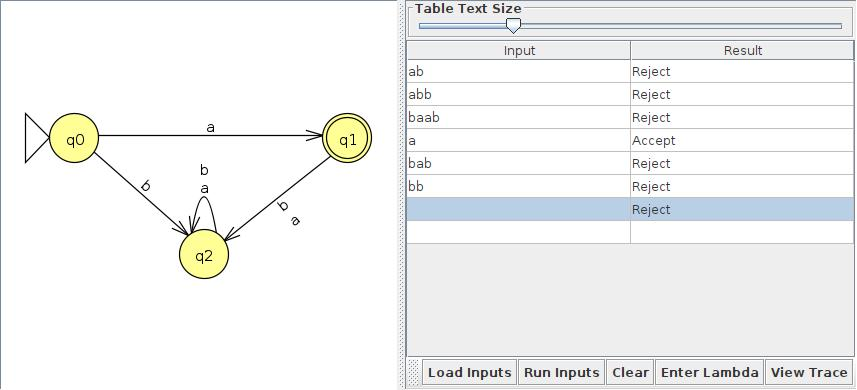
\includegraphics[width=\textwidth]{Automata.jpg}

\newpage
2. Finite automaton in Octave:

\begin{enumerate}[label=\alph{enumi})]
  \item Open the Octave finiteautomata.m script and test it with the given example (see script help) in the GitHub repository.
  \item Specify in finiteautomata.json the automaton created in Activity 1 and test it with the script!
  
\end{enumerate}

We start by testing the automata given in the example.

$>>$ finiteautomaton("aa*bb*","ab", "LaTeX")

$M = (\{q_0, q_1, q_2\}, \{a, b\}, \{(q_0, a, q_1), (q_1, a, q_1), (q_1, b, q_2), (q_2, b, q_2)\}, q_0, \{q_2\})$

$w = ab$

$(q_0, ab) \vdash (q_1, b) \vdash (q_2, \varepsilon)$

ans = 1
\\

This means that this automata recognizes the string "ab". Other tests return the following results:

a -$>$ ans = 0

abb -$>$ ans = 1

aba -$>$ ans = 0
\\

We will now test the automata that we designed in exercise 1.

$>>$finiteautomaton("Exercise1","a", "LaTeX")

$M = (\{q_0, q_1, q_2\}, \{a, b\}, \{(q_0, a, q_1), (q_0, b, q_2), (q_1, a, q_2), (q_1, b, q_2), (q_2, a, q_2), (q_2, b, q_2)\}, q_0, \{q_1\})$

$w = a$

$(q_0, a) \vdash (q_1, \varepsilon)$

ans = 1
\\

The string "a" is accepted by this automata. After testing the strings that we used in exercise 1 section b, we obtain the following results:

ab -$>$ ans = 0

abb -$>$ ans = 0

baab -$>$ ans = 0

a -$>$ ans = 1

bab -$>$ ans = 0

bb -$>$ ans = 0

$\varepsilon$ -$>$ ans = 0
\\

We can see that the automata defined in Octave behaves like the one designed in JFLAP.

\end{document}